\section{Android-sovellusten rakenne ja kehityssykli}

Tässä luvussa esitellään Androidin historiaa, kehitystyökaluja ja sovelluksen julkaisua sekä Android-sovellusten arkkitehtuuria ja pääkomponentit.

\subsection{Historia}

Androidin kehityksen aloitti Android Inc. -niminen yritys vuonna 2003. Google osti sen vuonna 2005. Kaksi vuotta myöhemmin, marraskuussa 2007 Androidin ensimmäinen versio julkaistiin ja samalla kerrottiin, että sen kehityksestä vastaa Open Handset Alliance, johon kuului Googlen lisäksi puhelinvalmistajia, kuten HTC ja Samsung, operaattoreita, kuten Sprint Nextel ja T-Mobile sekä komponenttivalmistajia, kuten Qualcomm ja Texas Instruments.

Ensimmäinen Androidille julkaistu kaupallinen laite oli HTC Dream -älypuhelin, joka julkaistiin lokakuussa 2008.
Loppuvuodesta 2010 Android nousi älypuhelinten markkinajohtajaksi. Syksyllä 2012 Androidilla oli jo tutkimuksesta riippuen 50-70 prosentin markkinaosuus ja laitevalikoima on kasvanut älypuhelimista muunmuassa tablet-tietokoneisiin, digibokseihin ja kameroihin \cite{wikiandroid}.

\subsection{Androidin kehitystyökalut}
\label{tools}

Android-sovelluksia tehdään pääsääntöisesti Java-ohjelmointikielellä. Google julkaisee Androidille ilmaista ohjelmistokehitystyökalua (Android SDK), joka kääntää sovelluksen ja pakkaa sen kuvien ja muiden resurssien kanssa apk-tiedostoksi (Android Application Package). Apk-tiedosto sisältää kaikki yhden sovelluksen asentamiseen tarvittavat tiedot. Android-sovelluksia ohjelmoidaan yleensä Eclipsellä, joka on suosittu ohjelmointiympäristö erityisesti Java-ohjelmistojen tekemiseen \cite{eclipse}. Android-sovellusten kehittämiseen tarvitsee käytännössä Javan kehitystyökaluista (SDK) version 5 tai uudemman, Androidin SDK:n, Eclipsen sekä Android-laajennoksen (Android Development Tools, ADT) Eclipselle \cite[25]{androidgamedev}.

Androidin SDK:n mukana tulee minimoitu versio Androidin järjestelmäkirjastoista, josta on mukana kirjastoluokkien rajapinnat, joiden avulla Eclipse osaa opastaa rajapintojen käytössä. Rajapinnan takana ei ole kuitenkaan oikeaa toteutusta, joten esimerkiksi yksikkötestit, jotka menevät kirjastoluokkiin asti, eivät toimi Eclipsestä Javalla ajettaessa.

Sovelluksen ja testien kehitysaikaista ajamista varten SDK:n mukana tulee Android-emulaattori. Emulaattoreita voi ajaa eri Android API:n versioilla ja laitteistoprofiileilla, jotta on mahdollista testata sovelluksen toimivuutta erilaisissa Android-ympäristöissä. Emulaattori kykenee myös jossain määrin simuloimaan lisälaitteiden, kuten kiihtyvyysanturin, toimintaa. Suurin puute emulaattorissa on sen heikko suoritusnopeus. Sovelluksia ja testejä voi ajaa kehitystyökalusta myös suoraan tietokoneeseen liitetyssä Android-laitteessa. 

Androidin Eclipse-laajennos toimii siltana Android SDK:n ja Eclipsen välillä mahdollistaen SDK:n tarjoamien ominaisuuksien hyödyntämisen suoraan Eclipsestä käsin. ADT:n avulla on myös mahdollista seurata tietokoneeseen kytkettyjen Android-laitteiden tapahtumalogeja ja debug-tietoja \cite[25-50]{androidgamedev}.

\subsection{Android-sovellusten rakenne}

Android on rakennettu Linuxin ytimen version 2.6 päälle ja koko Androidin järjestelmäkoodi on avointa, mikä tarkoittaa, että mikä tahansa valmistaja voi tehdä Androidin pohjalta oman mobiilikäyttöjärjestelmänsä. Esimerkiksi Amazon on julkaissut Kindle Fire -tabletteja oman Android-johdannaisen käyttöjärjestelmän päälle \cite{kindle_fire}. Jokainen sovellus on käyttäjänä järjestelmässä. Sovellusten oikeudet on rajattu siten, että ne pääsevät käsiksi vain kyseiseen sovellukseen liittyviin resursseihin. Sovelluksen ollessa käynnissä, se pyörii omana prosessina Linux-prosessien tavoin, jota Android-käyttöjärjestelmä hallitsee. Androidin turvallisuusratkaisu noudattaa vähimmän mahdollisen tiedon periaatetta: sovelluksella on vain ne oikeudet, joita se vähintään tarvitsee toimintaansa. Kaikkia ylimääräisiä oikeuksia varten täytyy erikseen pyytää lupa.

\begin{figure}[htb]
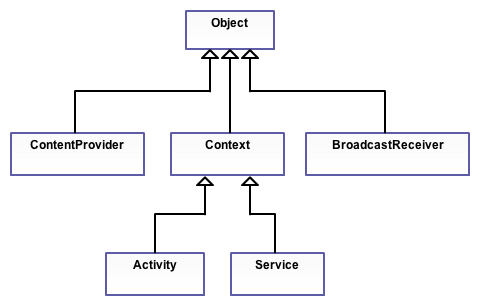
\includegraphics[width=130mm]{class_diagram.png}
\caption{Androidin tärkeimpien komponenttien luokkahierarkia} \label{class_diagram}
\end{figure}

Android-sovellukset koostuvat neljästä komponenttityypistä: aktiviteeteista (activities), palveluista (services), sisällöntarjoajista (content providers) sekä lähetysten vastaanottajista (broadcast receivers). Komponenttien välinen kommunikointi on pääosin tapahtumapohjaista; eri komponentit eivät keskustele suoraan keskenään, vaan kaikki siirtymät komponenttien välillä tapahtuvat käyttöjärjestelmän välittämien tapahtumaviestien perusteella. Tämän vaikutuksesta Android-sovellukset voivat helposti käyttää toiminnassaan järjestelmän ja toisten sovellusten tarjoamia komponentteja.

Kuvassa \ref{class_diagram} on esitelty Androidin peruskomponenttien muodostama luokkahierarkia. Vain aktiviteeteilla ja palveluilla on yhteinen yliluokka Context, lähetysten vastaanottajat ja sisällöntarjoajajat perivät vain Javan Object-luokan. Kuvaa on yksinkertaistettu siten, että Contextin ja Activityn ja Servicen välillä olevia Wrapper-luokkia on jätetty kuvaamatta perintähierarkiassa. Context-luokka tarjoaa aktiviteettien ja palveluiden käyttöön sovelluksen globaaliin tilaan liittyviä tietoja.

Aktiviteetti kuvaa yhtä sovelluksen käyttöliittymän kerrallaan muodostavaa näkymää. Sovelluksen käyttöliittymä koostuu useista aktiviteeteista, jotka muodostavat yhtenäisen sovelluksen, mutta jokainen aktiviteetti on toisistaan riippumaton. Eri sovellukset voivat myös käynnistää toistensa aktiviteetteja, mikäli vastaanottava sovellus sen sallii. Esimerkiksi kamera-sovellus voi käynnistää sähköposti-sovelluksen sähköpostinkirjoitus-aktiviteetin, jos ottamansa kuvan haluaa jakaa sähköpostilla. Aktiviteetit ovat Androidissa Activity-luokan aliluokkia.

Palvelut ovat taustaprosesseja, jotka suorittavat pitkäkestoisia operaatioita, kuten tiedon lataamista verkosta tai musiikin soittamista taustalla samalla, kun käyttäjä käyttää toista sovellusta. Palvelut eivät tarjoa käyttöliittymää ja toiset komponentit, kuten aktiviteetit, voivat käynnistää niitä. Palvelut ovat Service-luokan aliluokkia.

Sisällöntarjoajat vastaavat sovelluksen tarvitseman tiedon lukemisesta ja kirjoittamisesta pitkäkestoiseen muistiin. Tallennuspaikkana voi olla laitteen tiedostojärjestelmä, SQLite-tietokanta, verkko tai ylipäänsä mikä tahansa kohde, johon sovelluksella on luku- tai kirjoitusoikeudet. Sovellukset voivat käyttää toistensa sisällöntarjoajia, mikäli sovellus julkaisee ne muiden sovellusten käyttöön. Sisällöntarjoajat ovat ContentProvider-luokan aliluokkia.

Lähetysten vastaanottajat reagoivat järjestelmänlaajuisiin viesteihin ja tapahtumiin. Tällaisia ovat esimerkiksi ilmoitus, että akku on lopussa tai että käyttäjä on sulkenut tai avannut näytön. Ne voivat myös lähettää järjestelmänlaajuisia tapahtumaviestejä muille sovelluksille. Lähetysten vastaanottajat ovat BroadcastReceiver-luokan aliluokkia ja tapahtumat Intent-luokan aliluokkia.

Android-sovellukset käyttävät usein hyväkseen toisten sovellusten komponentteja. Sovellukset eivät pysty suoraan kutsumaan toisiaan. Halutessaan hyödyntää toisten sovellusten ominaisuuksia sovellus luo uuden aikeen, jonka järjestelmä välittää tiettyjen sääntöjen perusteella sopivalle vastaanottajalle (katso luku \ref{intents}). 

Android-sovelluksilla ei ole yksittäistä main-metodia, joka käynnistäisi ohjelman, kuten usein sovelluksissa on tapana. Sovellus voi sen sijaan käynnistyä vastaanottamansa aikeen johdosta monen eri komponentin kautta. Lisäksi sovellus saatetaan joutua käynnistämään ja sulkemaan useita kertoja esimerkiksi käyttäjän vaihtaessa puhelimen suuntausta tai vastaanotettaessa puhelua, joten sovelluksen pitää pystyä tehokkaasti palautumaan keskeytyneeseen tilaansa. Sovelluksella on siis lukuisia mahdollisia käynnistymis- ja sulkeutumispolkuja. Tämän takia ohjelmakomponenttien elinkaaren hallinta on tärkeä osa sovelluksen rakentamista.

Android-sovelluksilla on xml-muotoinen Manifest-tiedosto, jossa määritellään sovelluksen komponentit, niiden näkyvyys ja minkälaisia tapahtumia ne osaavat hallita. Manifestissa määritellään myös mitä rajoitteita sovellus asettaa käytettävissä olevalle Android-versiolle, puhelimen ominaisuuksille, kuten lisälaitteiden saatavuudelle ja näyttöresoluutiolle, ja mitä oikeuksia sovellus vaatii toimiakseen. Näin voidaan varmistaa, että sovellusta ei asenneta laitteelle, jossa ei ole sovelluksen välttämättä tarvitsemia ominaisuuksia \cite{android}.

\subsection{Aktiviteetit}

\begin{figure}[htb]
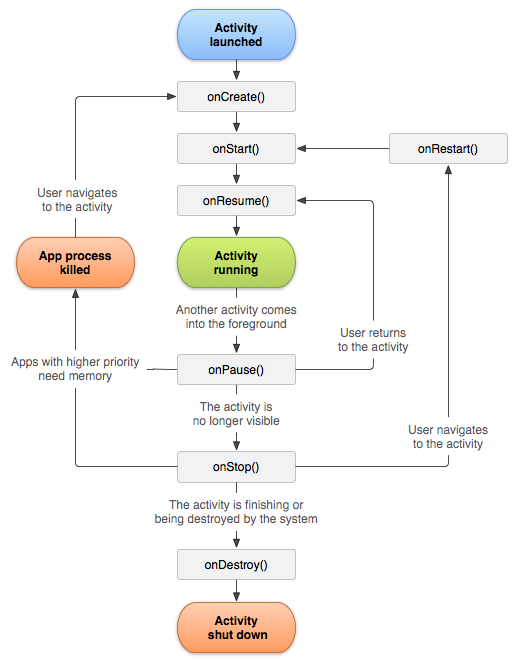
\includegraphics[width=110mm]{activity_lifecycle.png}
\caption{Aktiviteetin elinkaari \protect\cite{android}} \label{activity_lifecycle}
\end{figure}

Aktiviteetti kuvaa yhtä sovelluksen käyttöliittymän näkymää. Lähes aina aktiviteetti on koko näytön kokoinen - eli kaikki, mitä puhelimen ruudulla näkyy yläreunan status-palkkia lukuunottamatta on samaa aktiviteettia - mutta ne voivat olla myös pienempiä tai leijua osittain toisen aktiviteetin päällä. Kuitenkin vain yksi aktiviteetti kerrallaan voi olla aktiivinen - eli reagoida käyttäjän syötteisiin. Yksi sovelluksen aktiviteeteistä on yleensä pääaktiviteetti, joka käynnistyy silloin, kun käyttäjä avaa sovelluksen. 

Aktiviteettien elinkaaren hallinta on Android-sovelluksen kriittisimpiä osia, koska järjestelmän resurssit ovat yleensä hyvin rajalliset ja Android-laitteiden käyttöön liittyy tyypillisesti tiheä vaihtelu eri sovellusten välillä. Tällöin on tärkeää, että sovellus luovuttaa varaamansa resurssit muiden sovellusten käyttöön, kun sovellus vaihtuu, ja vastaavasti osaa palautua takaisin pysäytettäessä olleeseen tilaan käyttäjän palatessa sovellukseen. Nämä vaihdokset pitäisi lisäksi tapahtua mahdollisimman tehokkaasti, jotta järjestelmän toiminta olisi käyttäjän näkökulmasta mahdollisimman sulavaa sovellusten tilojen vaihtamisen yhteydessä.

Aktiviteetilla voi olla pitkäkestoisemmin kolme eri tilaa. Aktiviteetti on aktiivisessa tilassa (resumed) silloin, kun se on näytön etualalla ja käyttäjä käyttää juuri sitä aktiviteettia. Keskeytetyssä (paused) tilassa aktiviteetti on, kun se on osittain näkyvissä, mutta jokin toinen aktiviteetti on aktiivisena sen päällä. Keskeytetyt aktiviteetit ja niiden tilat pysyvät muistissa, joskin jos laitteen muisti on lopussa, järjestelmä saattaa tuhota sen. Aktiviteetti on pysäytetty (stopped) silloin, kun jokin toinen aktiviteetti peittää sen kokonaan näkyvistä. Tällainenkin aktiviteetti säilyy muistissa, jos laitteen resurssit ovat riittävät, mutta järjestelmä voi tuhota sen koska vain, jos resursseja tarvitaan muiden aktiviteettien käyttöön.

Aktiviteetin siirtyminen eri tilojen välillä tapahtuu järjestelmän kutsuessa aktiviteetin takaisinkutsumetodeita. Mahdolliset tilasiirtymäpolut näkyvät kuvassa \ref{activity_lifecycle}. 

Aktiviteetin koko elinkaari tapahtuu onCreate()- ja onDestroy()-kutsujen välillä. Aktiviteetin tulisi tehdä kaikki kerran suoritettavat tilanalustustehtävät kutsuttaessa onCreate()-metodia, kuten ulkoasun määrittely tai koko aktiviteetin elinkaaren ajan tarvittavan tiedonsiirtosäikeen avaus. Vastaavasti onDestroy()-kutsussa aktiviteetin tulisi vapauttaa kaikki loputkin aktiviteetin varaamat resurssit.

Aktiviteetin käyttäjälle näkyvä elinkaari on onStart()- ja onStop()-kutsujen välillä. onStart()-metodia kutsutaan, kun aktiviteetti tulee näkyväksi käyttäjälle, ja onStop()-metodia kutsutaan, kun jokin toinen aktiviteetti on peittänyt kyseisen aktiviteetin kokonaan. Näkyvän elinkaaren aikana tulisi ylläpitää niitä resursseja, joita tarvitaan käyttäjän kanssa kommunikointiin sekä sellaisia, jotka saattavat muuten vaikuttaa käyttäjälle näkyvään käytöliittymään. Esimerkiksi lähetystenvastaanottajaa on hyvä kuunnella tällä välillä mahdollisten järjestelmänlaajuisten käyttöliittymään vaikuttavien tapahtumien varalta. onStart() ja onStop() -kutsuja voi tulla lukuisia aktiviteetin koko elinkaaren aikana. onRestart()-metodia kutsutaan, jos aktiviteetti on jo luotu aiemmin ja pysäytetty sitten onStop()-kutsulla. onRestart()-kutsua seuraa aina onStart()-kutsu.

Aktiviteetti on aktiivisena näytön etualalla onResume() ja onPause() -kutsujen välillä. Kun aktiviteetti on etualalla, käyttäjä käyttää juuri sitä ja se on kaikkien muiden aktiviteettien päällä. onResume() ja onPause() -kutsuja voi tulla tiheästi, esimerkiksi aina kun laitteen näyttö menee lepotilaan tai tulee jokin ilmoitus aktiviteetin päälle, joten niiden toteutus ei saa olla liian raskas.

Androidin järjestelmä voi tuhota sovelluksen prosessin onPause()-, onStop()- tai onDestroy()-kutsun jälkeen. Tämän takia pysyväksi tarkoitettu tieto on tallennettava onPause()-kutsun jälkeen. Tallennus voidaan tehdä esimerkiksi toteuttamalla takaisinkutsumetodi onSaveInstanceData(), jota kutsutaan aina, ennen kuin järjestelmä mahdollistaa aktiviteetin tuhoamisen. onSaveInstanceData() saa parametrinaan Bundle-olion, johon voi tallentaa tietoja nimi-arvo-pareina. Sama Bundle-olio tulee aktiviteetille onCreate() ja onRestoreInstanceState() -metodeille. Tiedon palautuksen voi tehdä kummassa tahansa näistä metodeista. Activity-luokka tarjoaa myös oletustoteutuksen onSaveInstanceData() ja onRestoreInstanceState()-metodeista, jotka osaavat monissa tapauksissa suorittaa tiedon tallennuksen ja palautuksen. Aktiviteetin tilanpalautusta tarvitaan usein, esimerkiksi aina kun käyttäjä vaihtaa sovelluksen suuntaa pysty- ja vaakasuuntien välillä.

Aktiviteettien vaihtumisen yhteydessä takaisinkutsujen järjestys on aina sama. Kun aktiviteetti A käynnistää aktiviteetti B:n, ensin kutsutaan aktiviteetti A:n onPause()-metodia, sitten aktiviteetti B:n onCreate(), onStart() ja onResume()-metodeita peräkkäin. Viimeiseksi kutsutaan aktiviteetti A:n onStop()-metodia, mikäli aktiviteetti B peittää sen kokonaan. Näin esimerkiksi aktiviteetti A:n onPause()-metodissa tietokantaan tallennetut tiedot ovat käytössä aktiviteetti B:tä käynnistettäessä. Jos muutoksia taas tekee onStop()-metodissa, ne tapahtuvat vasta aktiviteetti B:n käynnistyttyä \cite{android}.

\subsection{Palvelut}

\begin{figure}[htb]
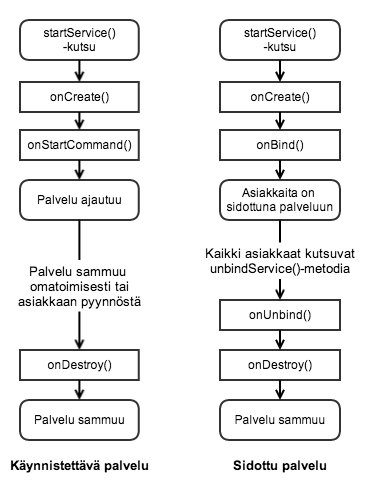
\includegraphics[width=100mm]{service_lifecycle.png}
\caption{Palvelun elinkaari \protect\cite{android}} \label{service_lifecycle}
\end{figure}

Palvelut ovat pitkäkestoisia taustaoperaatioita. Muut sovelluskomponentit voivat käynnistää niitä, ja ne jatkuvat vaikka käyttäjä lopettaisi kyseisen sovelluksen käyttämisen. Palvelu voi esimerkiksi soittaa musiikkia, suorittaa verkkotransaktioita, kommunikoida sisällöntarjoajien kanssa tai tehdä levykirjoitusta.

Palveluita on kahdenlaisia. Käynnistettävät (\emph{started}) palvelut suorittavat tehtävänsä kun niiden startService()-metodia kutsutaan. Tällainen palvelu voi jatkaa pyörimistä taustalla, vaikka sovellus suljettaisiin. Tyypillisesti käynnistettävä palvelu tekee jonkin yhden operaation, kuten tiedoston latauksen tai lähettämisen, ja lopettaa sitten itsensä. Käynnistettävät palvelut eivät yleensä palauta palautusarvona kutsujalle mitään. Käynnistettävien palveluiden tulee sulkea itsensä operaation valmistuttua kutsumalla stopSelf()-metodia. Myös muut komponentit voivat sulkea palvelun kutsumalla stopService()-metodia.

Sidotut (\emph{bound}) palvelut ovat sellaisia, että sovelluskomponentit sitovat palvelun niihin kutsumalla bindService()-metoida. Sidotut palvelut tarjoavat asiakas-palvelin-rajapinnan sitovalle komponentille. Palvelu voi vastaanottaa pyyntöjä ja palauttaa vastauksia niihin. Palvelun elinkaari on sama kuin sen sitoneen komponentin. Useampi komponentti voi sitoa saman palvelun yhtä aikaa. Tällöin palvelu sulkeutuu kun viimeinenkin niistä lopettaa toimintansa. Sitominen vapautetaan kutsumalla unbindService()-metodia.

Useimmiten käynnistettävät ja sidotut palvelut ovat erillisiä, mutta joissain tilanteissa sama palvelu voi toimia sekä käynnistettävänä että sidottuna palveluna. Käynnistettäviä palveluita käytetään tyypillisesti pitkäkestoisiin taustaoperaatioihin, jotka suoritetaan taustalla ilman että käyttäjä puuttuu niiden toimintaan. Sidotut palvelut taas voivat tarjota sovellukselle minkä tahansa palvelurajapinnan, jonka kanssa sovellus voi kommunikoida palvelun elinkaaren ajan.

Palveluiden elinkaari on esitetty kuvassa \ref{service_lifecycle}. Aktiviteettien tavoin koko palvelun elinkaari tapahtuu onCreate() ja onDestroy()-kutsujen välissä ja palvelun alustus tapahtuu onCreate()-metodissa. Sidotun palvelun aktiivinen elinkaari on onBind() ja onUnbind()-kutsujen välillä. Käynnistettävän palvelun elinkaari puolestaan alkaa onStartCommand()-kutsusta kunnes se sulkee itsensä stopSelf()-kutsulla. onBind() ja onStartCommand() -metodit saavat parametrinaan aikeen, jonka niitä kutsunut komponentti antoi bindService() tai startService() -metodille \cite{android}.

\subsection{Sisällöntarjoajat}

Sisällöntarjoajat tarjoavat pääsyn pysyvästi tallennettuun tietoon. Ne kapsuloivat tiedon ja tarjoavat mekanismit tiedon yksityisyyden hallintaan. Sisällöntarjoajat toimivat rajapintana tiedon ja sovelluskoodin välillä. Kun sisällöntarjoajan tietoon halutaan päästä käsiksi, käytetään ContentResolver-oliota Context-luokassa, joka sitten kommunikoi itse sisällöntarjoajan kanssa.

Sisällöntarjoajat eivät ole välttämättömiä sovelluksessa, jos sovelluksen säilömään tietoon ei tarvitse päästä käsiksi sovelluksen ulkopuolelta. Sovellustenväliseen kommunikointiin sisällöntarjoajat tarjoavat vakiorajapinnan, joka pitää huolen prosessienvälisestä kommunikoinnista ja tietoturvallisuudesta.

Androidin mukana tulee valmiiksi toteutetut sisällöntarjoajat esimerkiksi musiikille, videotiedostoille ja käyttäjän yhteystiedoille. Nämä sisällöntarjoajat ovat kaikkien sovellusten käytettävissä \cite{android}.

\subsection{Aikeet}
\label{intents}

Suurin osa Android-sovellusten kommunikaatiosta on tapahtumapohjaista. Niin aktiviteetit, palvelut kuin sisällöntarjoajatkin käynnistetään lähettämällä niille aie (\emph{intent}). Tapahtumia käytetään Androidissa, koska niiden avulla komponentit voidaan sitoa toisiinsa ajonaikaisesti ja vasta silloin, kun niitä varsinaisesti tarvitaan. Itse aie-oliot ovat passiivisia tietorakenteita, joissa on abstrakti kuvaus operaatiosta, joka halutaan suoritettavan, tai lähetysten (\emph{broadcast}) tapauksessa kuvaus siitä, mitä on tapahtunut. 

Aikeiden kohde voidaan nimetä ekspliittisesti ComponentName-kentässä. Tällöin annetaan kohdekomponentin täydellinen nimi paketteineen, jolloin kohde voidaan tunnistaa yksikäsitteisesti. Tämän muodon käyttäminen vaatii, että kutsuva komponentti tietää kohdekomponentin nimen. Sovelluksensisäisessä kommunikoinnissa tämä onnistuu, mutta sovellustenvälisessä kommunikoinnissa useinkaan ei. Tällöin kohde päätellään implisiittisesti muista aikeelle annetuista kentistä.

Action-kentässä annetaan tapahtuma, joka aikeella halutaan käynnistää, esimerkiksi puhelun aloitus, tai lähetysten vastaanottajien tapauksessa järjestelmässä tapahtunut tapahtuma, kuten varoitus akun loppumisesta. Intent-luokassa määritellään lukuisia vakioita erilaisia tapahtumia varten, mutta niiden lisäksi sovellukset voivat määritellä myös omia tapahtumia.

Data-kentässä annetaan tapahtumaan liittyvän tiedon osoite (\emph{URI}) ja tyyppi (\emph{MIME}). Näin vastaanottava komponentti tietää minkätyyppistä tietoa aikeeseen liittyy, ja mistä se löytyy. Category-kentässä kerrotaan, minkä tyyppisen komponentin odotetaan käsittelevän aikeen. Näitäkin Intent-luokka tarjoaa valmiita, mutta omien käyttö on mahdollista.

Aikeen vastaanottava komponentti voidaan päätellä kahdella tavalla. Komponentti valitaan ekplisiittisesti, jos ComponentName-kentässä on arvo. Tällöin muiden kenttien arvoista ei välitetä. Muussa tapauksessa Action-, Data- ja Category-kenttien arvojen perusteella selvitetään, mitä soveltuvia vastaanottavia komponentteja järjestelmään on asennettuna. Tässä käytetään apuna aiesuotimia (\emph{intent filter}).

Sovellukset voivat määritellä aiesuotimia, jotta järjestelmä tietää, mitkä sovellukset voivat ottaa vastaan aikeita. Aiesuotimet ovat komponenttikohtaisia, ja ne määrittelevät, mitä tapahtumia, tietotyyppejä ja kategorioita ne tukevat. Aiesuotimia käytetään hyväksi implisiittisessä kohteen määrittelyssä. Jos kohde on määritelty eksplisiittisesti komponentin nimellä, aiesuotimilla ei ole vaikutusta \cite{android}.

\subsection{Android manifest}

Jokaisella Android-sovellukseen kuuluu AndroidManifest.xml-tiedosto, joka sisältää järjestelmälle välttämätöntä tietoa sovelluksen ajamiseksi. Manifestissa määritellään sovelluksen Java-paketti, joka toimii samalla sovelluksen yksilöllisenä tunnisteena. Manifestissa on myös listattu sovelluksen komponentit, aktiviteetit, palvelut, sisällöntarjoajat ja lähetysten vastaanottajat, joista sovellus koostuu, sekä niiden toiminnallisuus ulkopuolelta tulevien aikeiden kannalta Lisäksi manifestissa ilmoitetaan, mitä oikeuksia sovellus tarvitsee toimiakseen sekä mitä oikeuksia toisilla sovelluksilla pitää olla, jotta ne voivat käyttää kyseisen sovelluksen palveluita. Näiden tietojen lisäksi manifestissa määritellään sovelluksen vaatimuksen ympäristöltään: mikä on sovelluksen vaatima Android APIn minimiversio sekä mitä kirjastoja sovellus tarvitsee toimiakseen \cite{android}.

Jos sovellus tarvitsee välttämättä laitteelta tiettyjä ominaisuuksia, on mahdollista suodattaa sovellus pois Androidin sovelluskaupan hauista, jos sitä haetaan laitteella, joka ei tue sovelluksen vaatimia ominaisuuksia. Tärkeimmät suotimet ovat androidin API:n minimiversio, tiettyjen lisälaitteiden olemassaolo ja näytön koko.

<uses-sdk>-direktiivillä (\emph{directive}) määritellään Androidin APIn minimiversio. Jos laitteessa on käytössä pienempi API-versio kuin direktiivillä annettu, sovellusta ei näytetä hakutuloksissa. <support screens>-direktiivi määrittelee, millä näytön koolla sovellus toimii. Tavallisesti määrittelemällä jokin tuettu koko, sovelluskauppa olettaa, että laite tukee sen lisäksi myös isompia näyttökokoja, muttei pienempiä. On myös mahdollista määritellä erikseen kaikki tuetut näyttökoot.

<uses-feature>-direktiivillä voidaan määritellä mitä ominaisuuksia sovellus vaatii. Näitä on sekä laitteistotasolla, kuten kamera, kiihtyvyysanturi tai kompassi, että ohjelmistotasolla, kuten vaikka liikkuvat taustakuvat, joiden pyörittämiseen kaikissa Android-laitteissa ei riitä resursseja. <uses-feature>-direktiiviä käytetään, kun sovellus ei lainkaan toimi ilman kyseistä ominaisuutta \cite{android_compatibility}.

\subsection{Android-sovelluksen julkaiseminen}

\begin{figure}[htb]
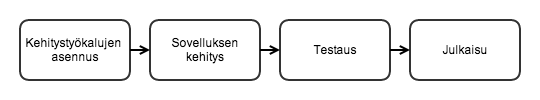
\includegraphics[width=130mm]{kehityskaari.png}
\caption{Android-sovelluksen kehityskaari \protect\cite{android}} \label{publishing_overview}
\end{figure}

Kuvassa \ref{publishing_overview} on kuvattu yksinkertaistettu Android-sovelluksen kehityskaari. Kun sovellus on kehitetty ja testattu, on viimeisenä vaiheena sen julkaisu. Android-sovellukset julkaistaan yleensä Google Play -sovelluskaupassa \cite{google_play}. Sovelluksia voi julkaista kuka tahansa. Julkaistaakseen sovelluksia julkaisijan täytyy rekisteröityä ja maksaa 25 dollarin rekisteröitymismaksu. Sovelluksen voi julkaista halutessaan myös vaikka omilla verkkosivuillaan tai muissa sovelluskaupoissa, mutta parhaan näkyvyyden Android-laitteissa saa tällä hetkellä Google Playssa.

Julkaisua varten sovellus täytyy konfiguroida julkaisua varten ja kääntää julkaistava APK-tiedosto, joka ladataan sovelluskauppaan. Lisäksi tarvitaan sovelluskauppaa varten muutama ruutukaappaus sovelluksesta sekä esittelyteksti. Sovellukselle pitää myös valita nimi. Sovellus voi olla joko ilmainen tai maksullinen ja siinä voi olla lisäksi sovelluksen sisäisiä maksumekanismeja. Ainut rajoitus on, että kerran ilmaisena julkaistua sovellusta ei saa muuttaa maksulliseksi. Ilmaisiseksi ladattavissakin sovelluksissa voi kuitenkin käyttää sovelluksen sisäisiä maksumekanismeja.

Sovelluksen voi julkaista vain haluamissaan maissa ja saatavuutta voi rajoittaa myös laitekohtaisesti tai Androidin version perusteella. Google Play mahdollistaa myös alfa- ja betatestauksen pienille ryhmille. Kehittäjän hallintanäkymästä näkee tilastotietoa sovelluksen kaatumisista ja virhetilanteista sekä mitä versioita sovelluksesta on käytössä ja missä Androidin versioissa niitä ajetaan. Sovelluksesta voi tehdä milloin tahansa päivitysversion lataamalla päivitetyn APK-tiedoston sovelluskauppaan. Google Play ilmoittaa sovelluksen ladanneille automaattisesti uuden version ilmestymisestä.